\chapter{Wdrożenie i testy}

\section{Wdrożenie}
System został wdrożony 1 maja 2023 roku. Wdrożenie polegało na uruchomieniu serwera z bazą danych, jedną stację przekaźnikową oraz uruchomieniu 3 urządzeń pomiarowych.

\subsection{Węzły sieci}
% Węzły sieci zostały umieszczone w trzech różnych miejscach w Lublinie. Pierwszy z nich został umieszczony na dachu budynku Wydziału Matematyki, Fizyki i Informatyki UMCS. Drugi został umieszczony na dachu budynku Wydziału Elektrotechniki i Informatyki Politechniki Lubelskiej. Trzeci został umieszczony na dachu budynku Wydziału Informatyki Politechniki Lubelskiej. Wszystkie urządzenia zostały umieszczone na wysokości 20 metrów nad poziomem gruntu. Wszystkie urządzenia zostały umieszczone na zewnątrz, w~specjalnych obudowach, które zapewniają ochronę przed warunkami atmosferycznymi. Wszystkie urządzenia zostały zasilone z sieci elektrycznej.

Trzy węzły sieci zostały rozmieszczone na małym obszarze, około 30 metrów od siebie, w dwóch budynkach. Dwa urządzenia (jedno Raspberry Pi Pico i jedno TTGO LoRa32) zasilane są z sieci, jedno za pomocą baterii. Urządzenia zostały połączone z czujnikami za pomocą zwykłych kabli prototypowych, jak na zdjęciu~\ref{rys:wezel1} i ~\ref{rys:wezel2}. Przykład urządzenia wykorzystującego wbudowane czujniki został zaprezentowany na zdjęciu~\ref{rys:wezel2}

\begin{figure}[b!]
    \begin{center}
        % 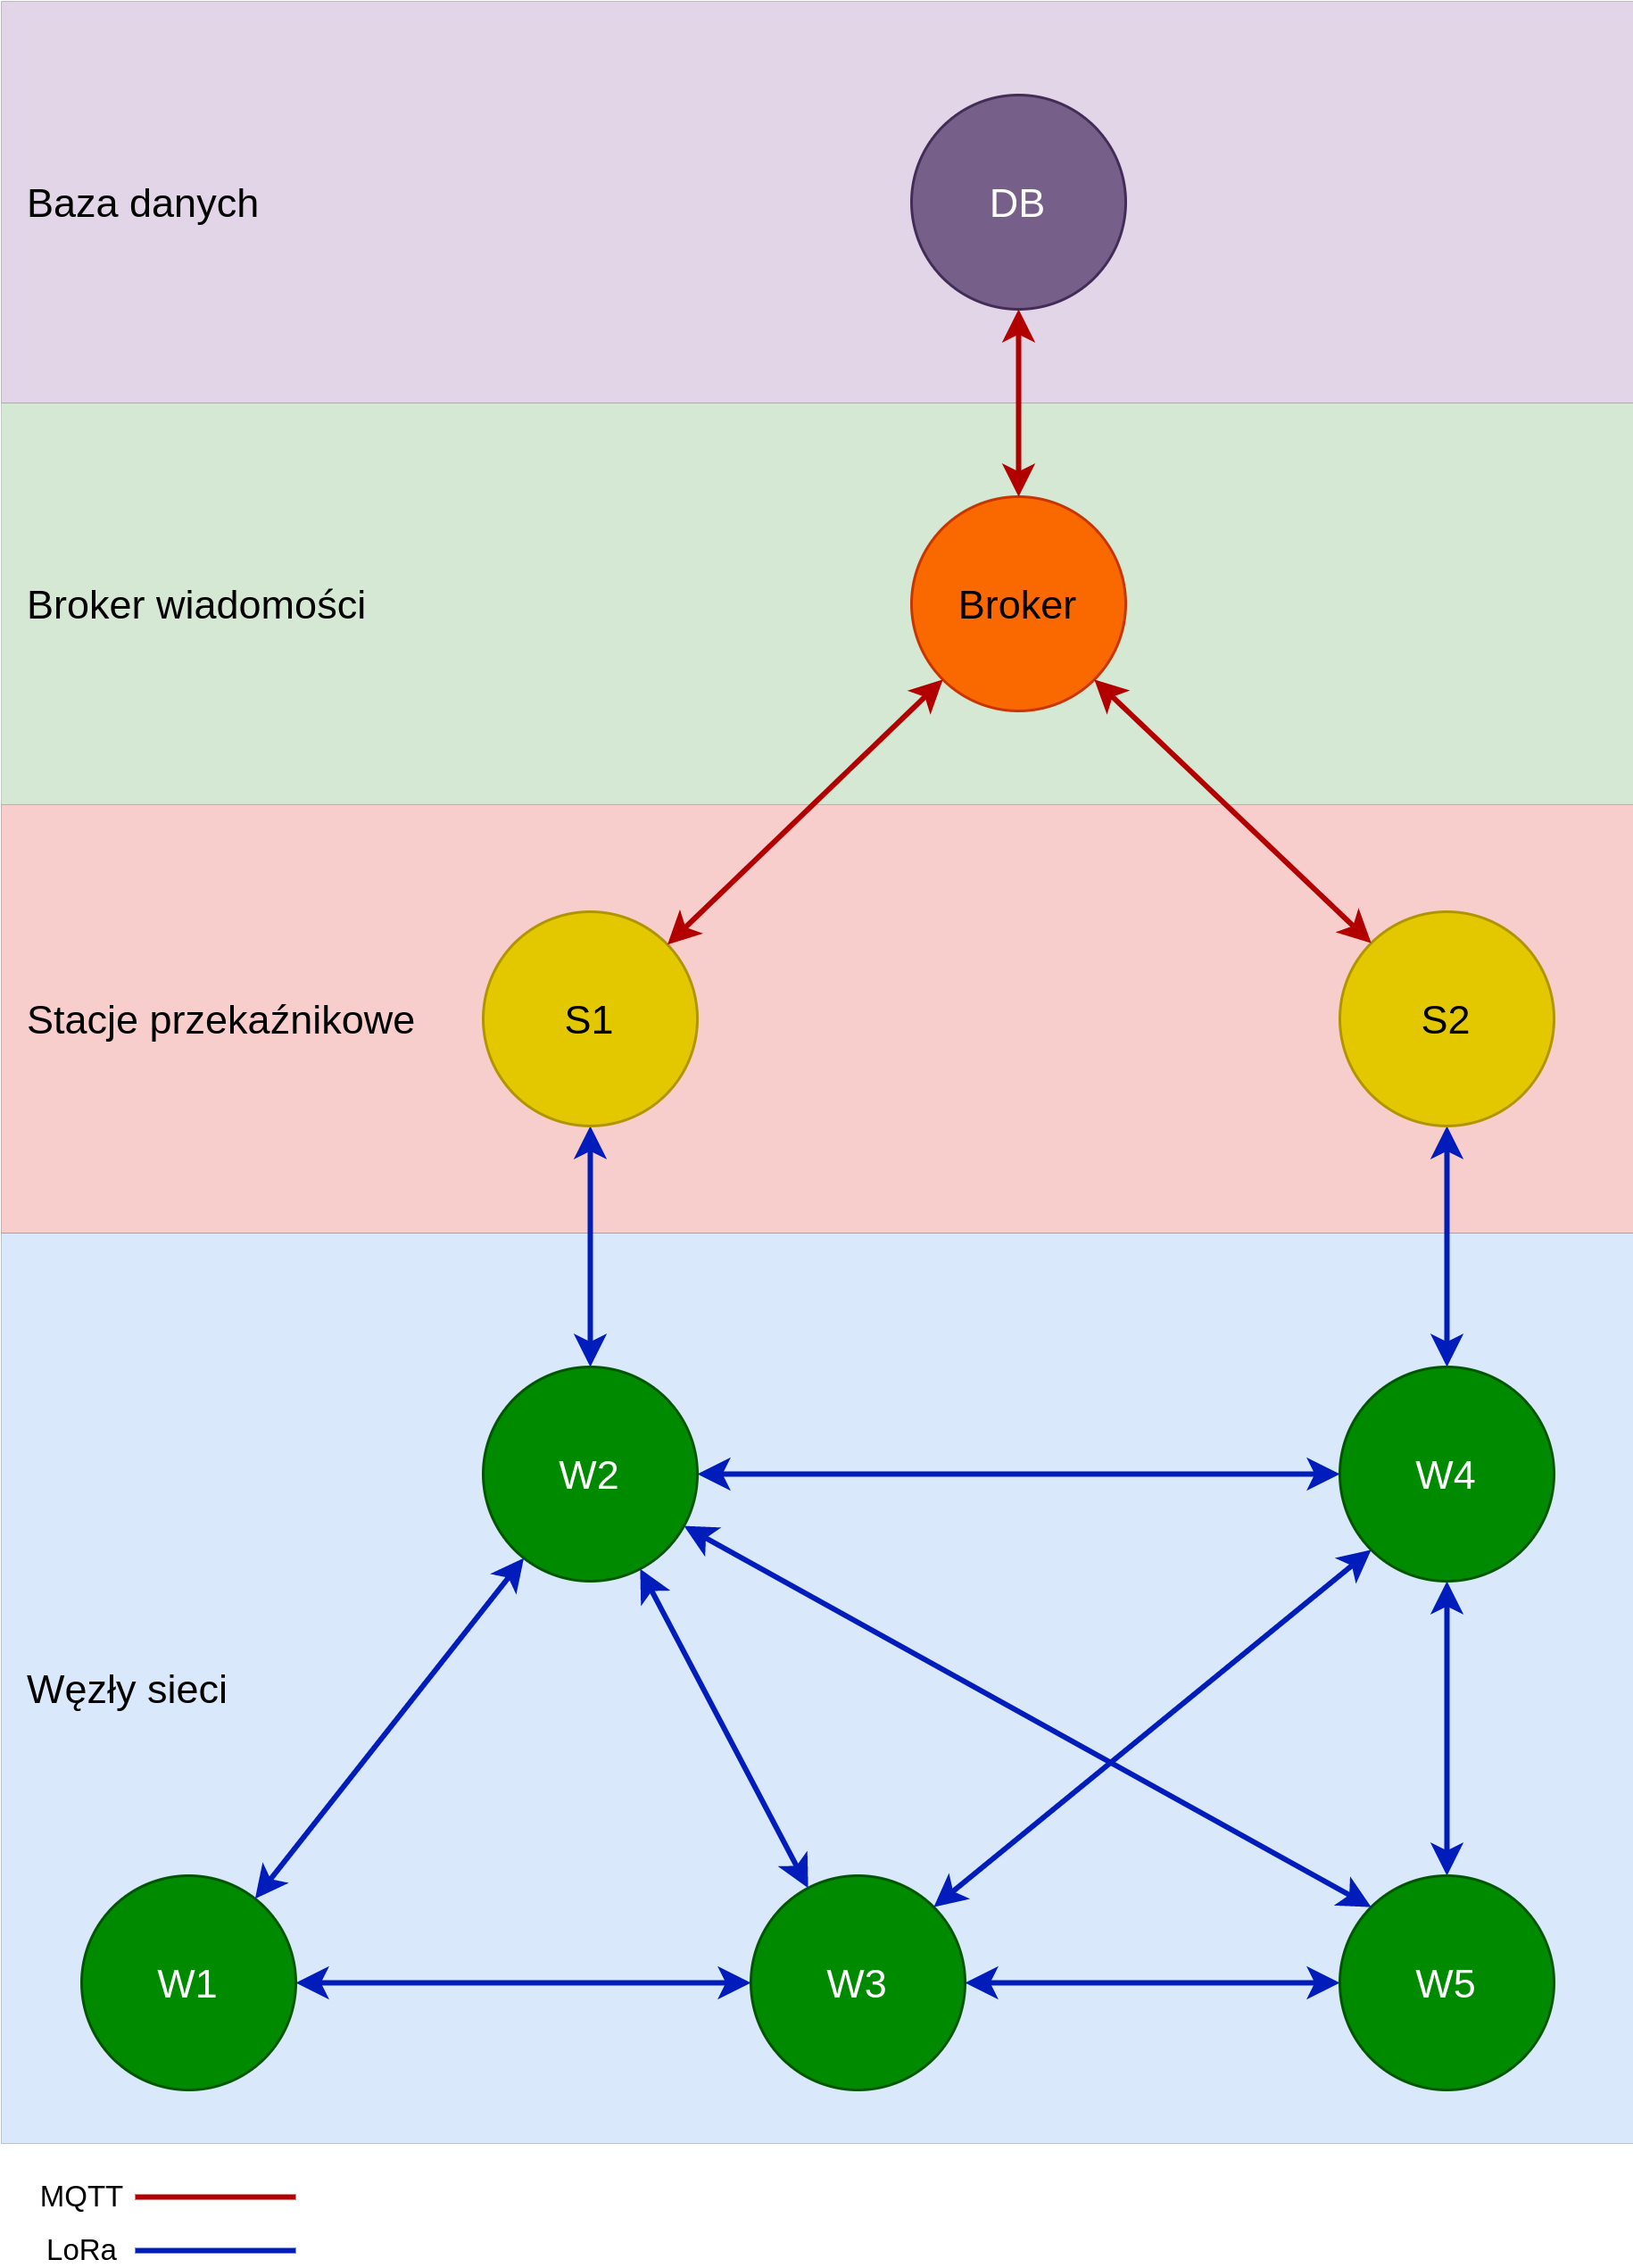
\includegraphics[width=3cm]{pic/diagram-systemu.png}
        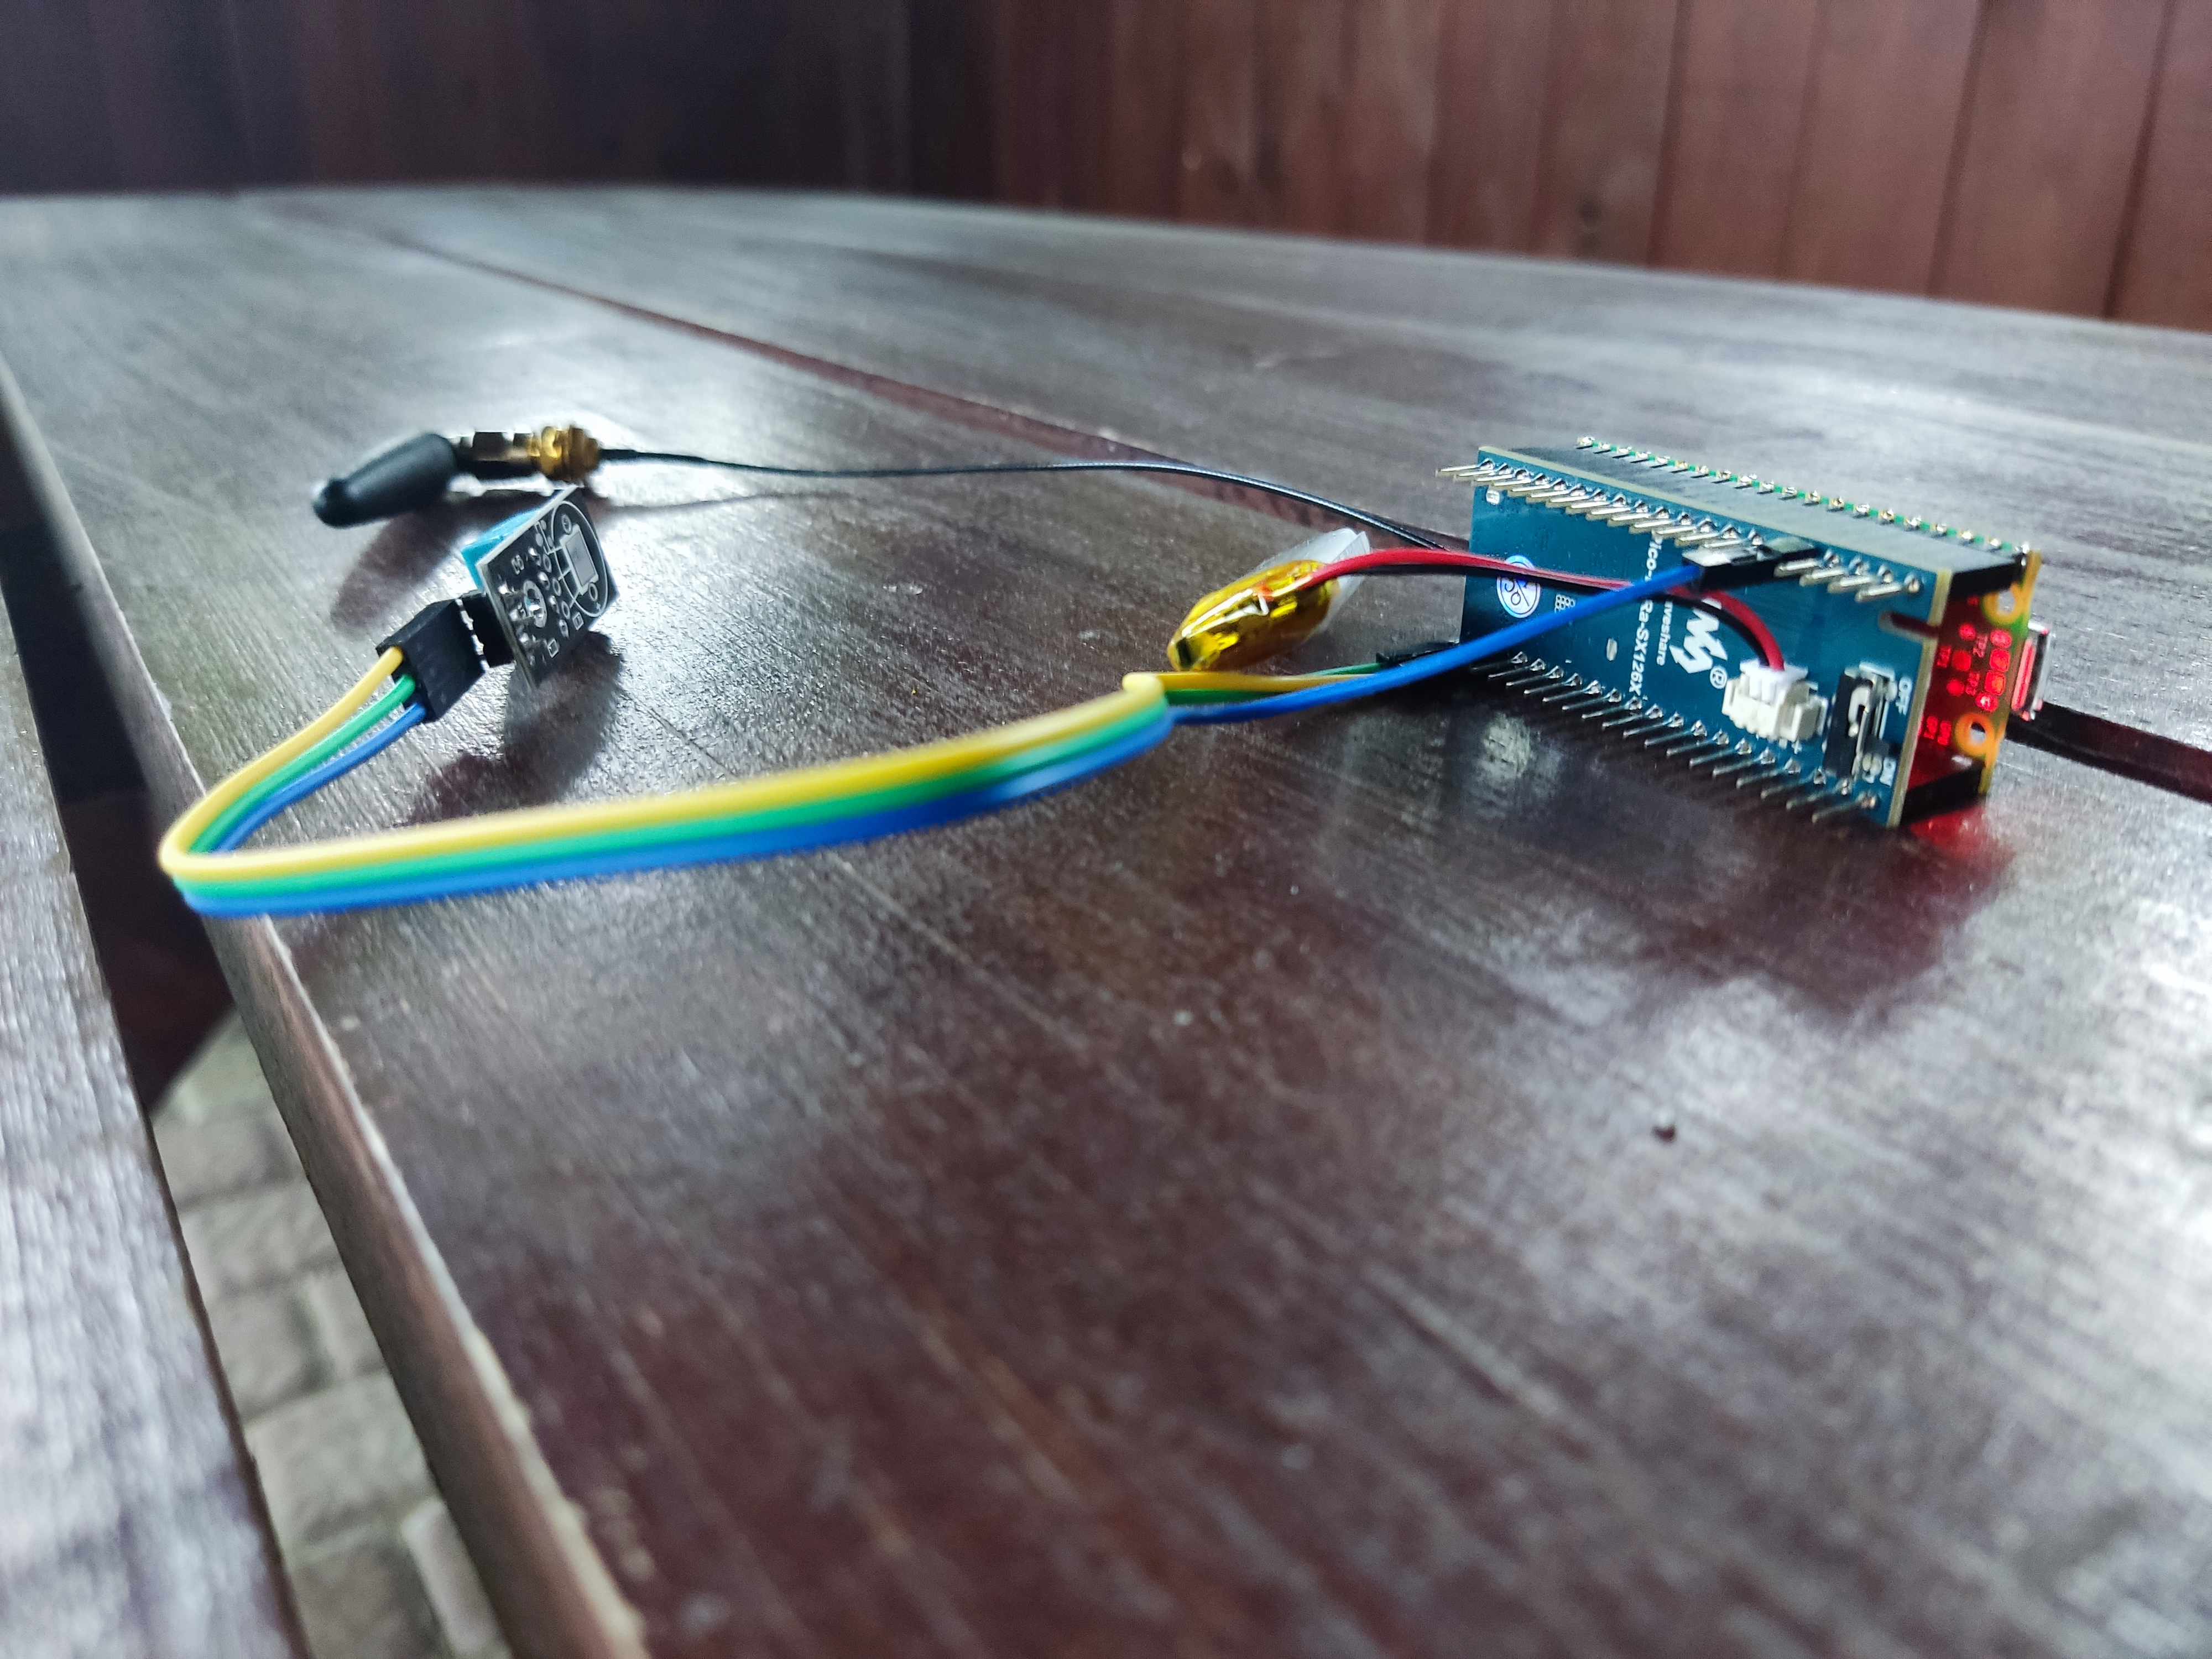
\includegraphics[width=13cm]{pic/wezel1.jpg}
    \end{center}
    \caption{Zdjęcie węzła sieci opartego o Raspberry Pi Pico wraz z baterią}\label{rys:wezel1}
\end{figure}

\begin{figure}[b!]
    \begin{center}
        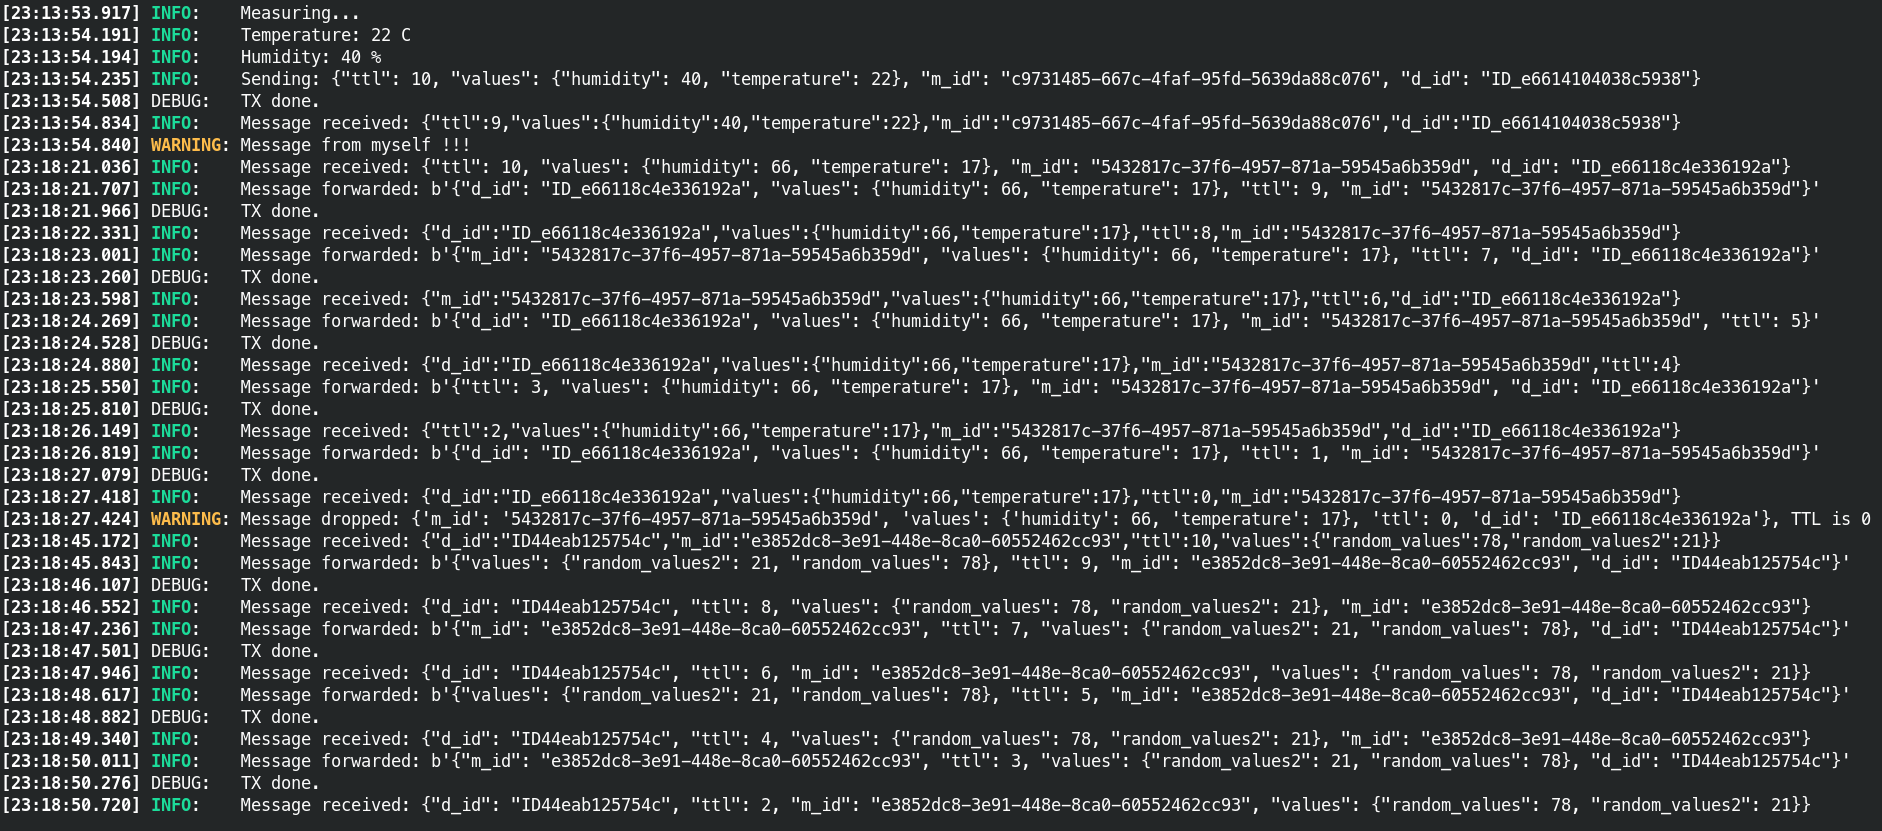
\includegraphics[width=13cm]{pic/logi-pico.png}
        % 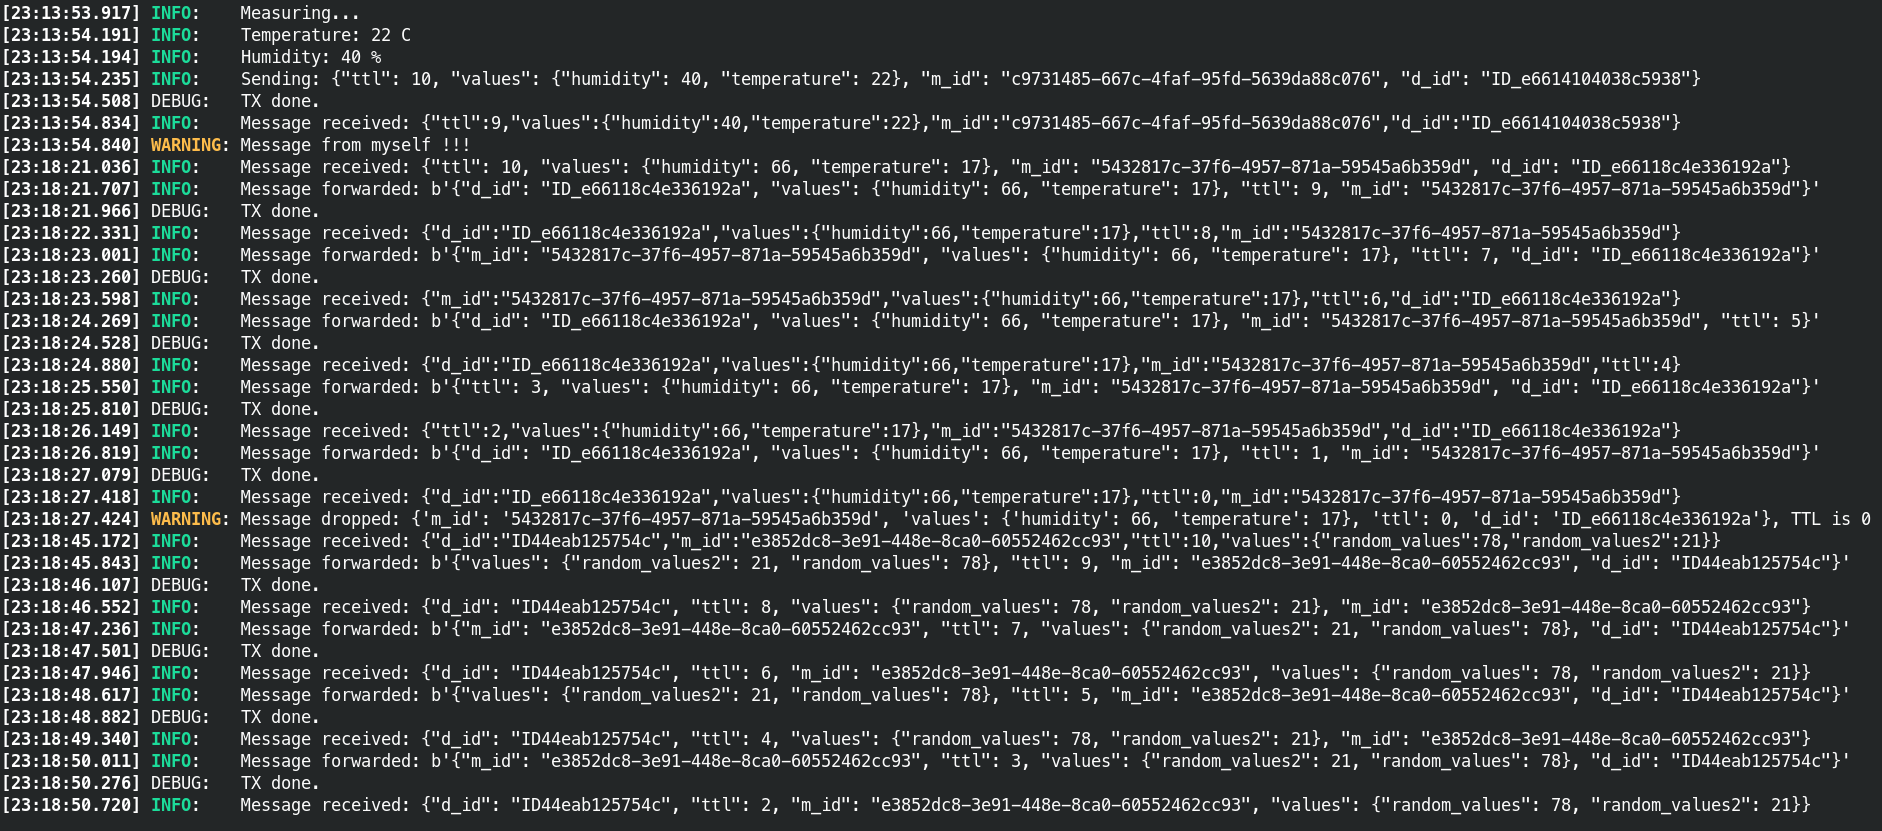
\includegraphics[height=13cm]{pic/logi-pico.png}
    \end{center}
    \caption{Zrzut ekranu zawierający logi z jedno z węzłów sieci(Raspberry Pi Pico)}\label{rys:logi-pico}
\end{figure}

\begin{figure}[b!]
    \begin{center}
        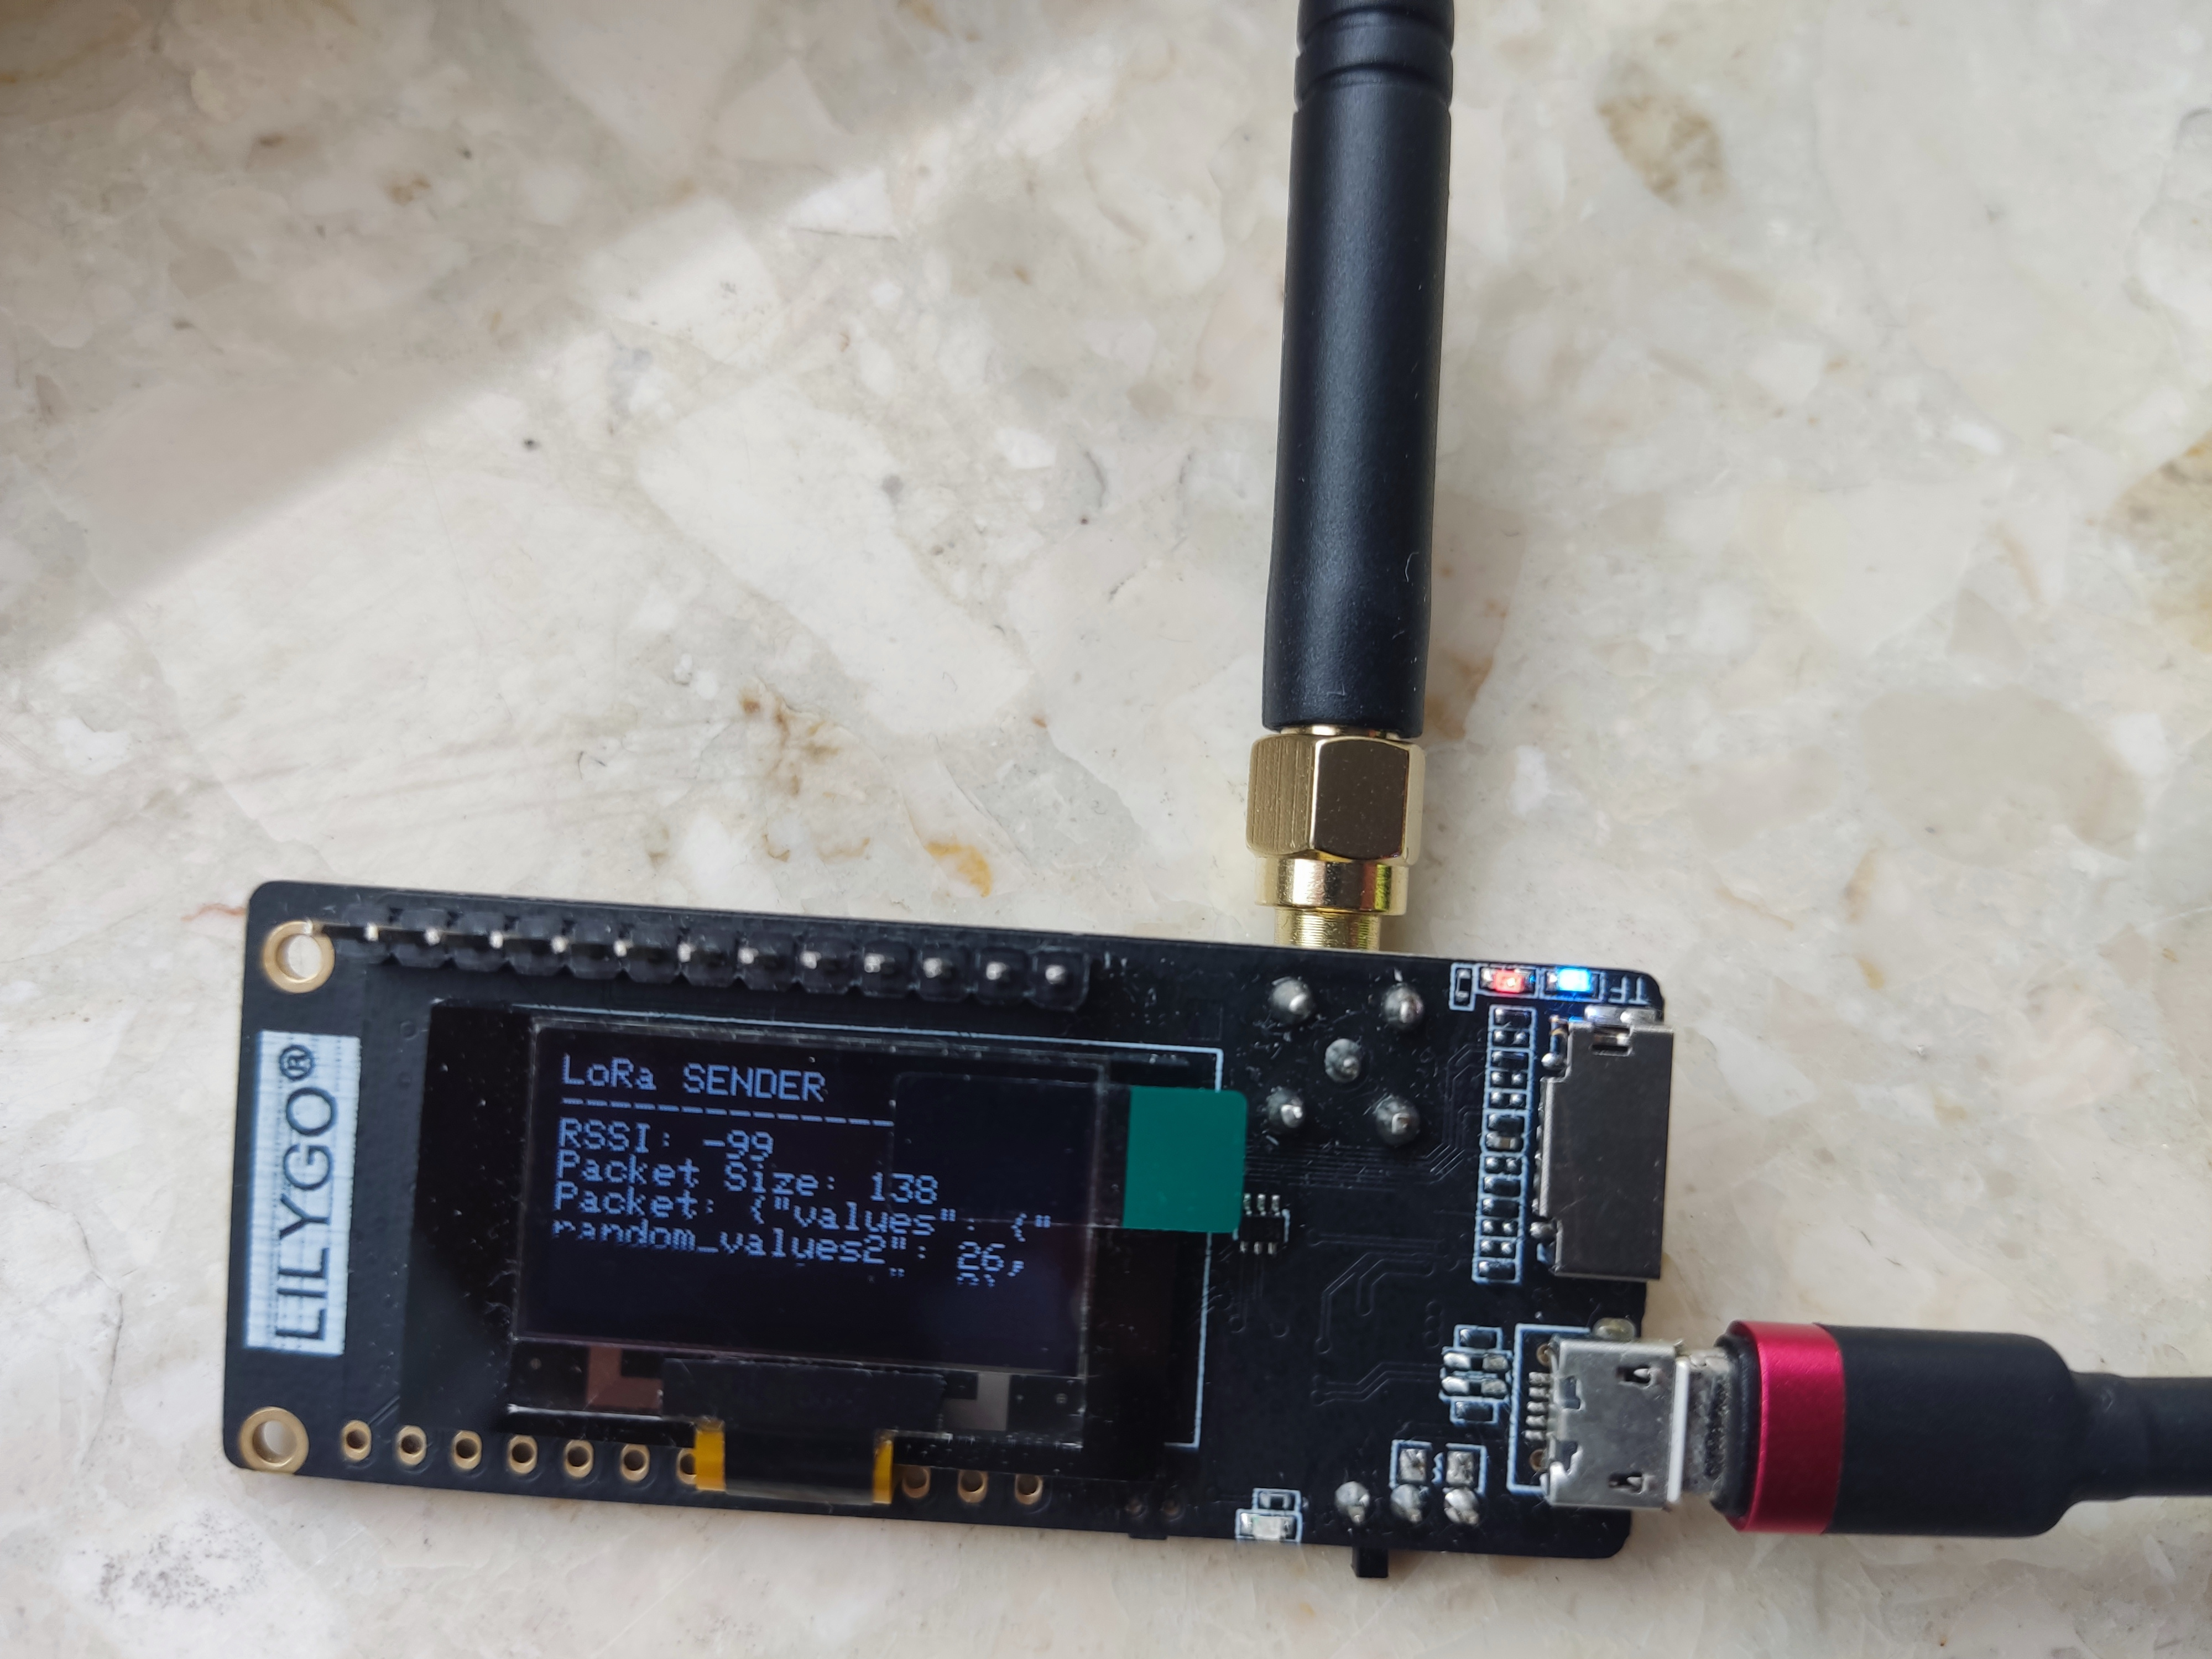
\includegraphics[width=13cm]{pic/wezel2.jpg}
    \end{center}
    \caption{Zdjęcie węzła sieci opartego  TTGO LoRa32}\label{rys:wezel2}
\end{figure}

\subsection{Stacja przekaźnikowa}
Stacja przekaźnikowa została umieszczona w pobliżu głównego serwera, w zasięgu sieci WiFi, wewnątrz budynku. Urządzenie zostało zasilone z sieci elektrycznej. Na ekranie urządzenia wyświetlane są informacje o stanie urządzenia, jak na zdjęciu~\ref{rys:stacja1}.

\begin{figure}[b!]
    \begin{center}
        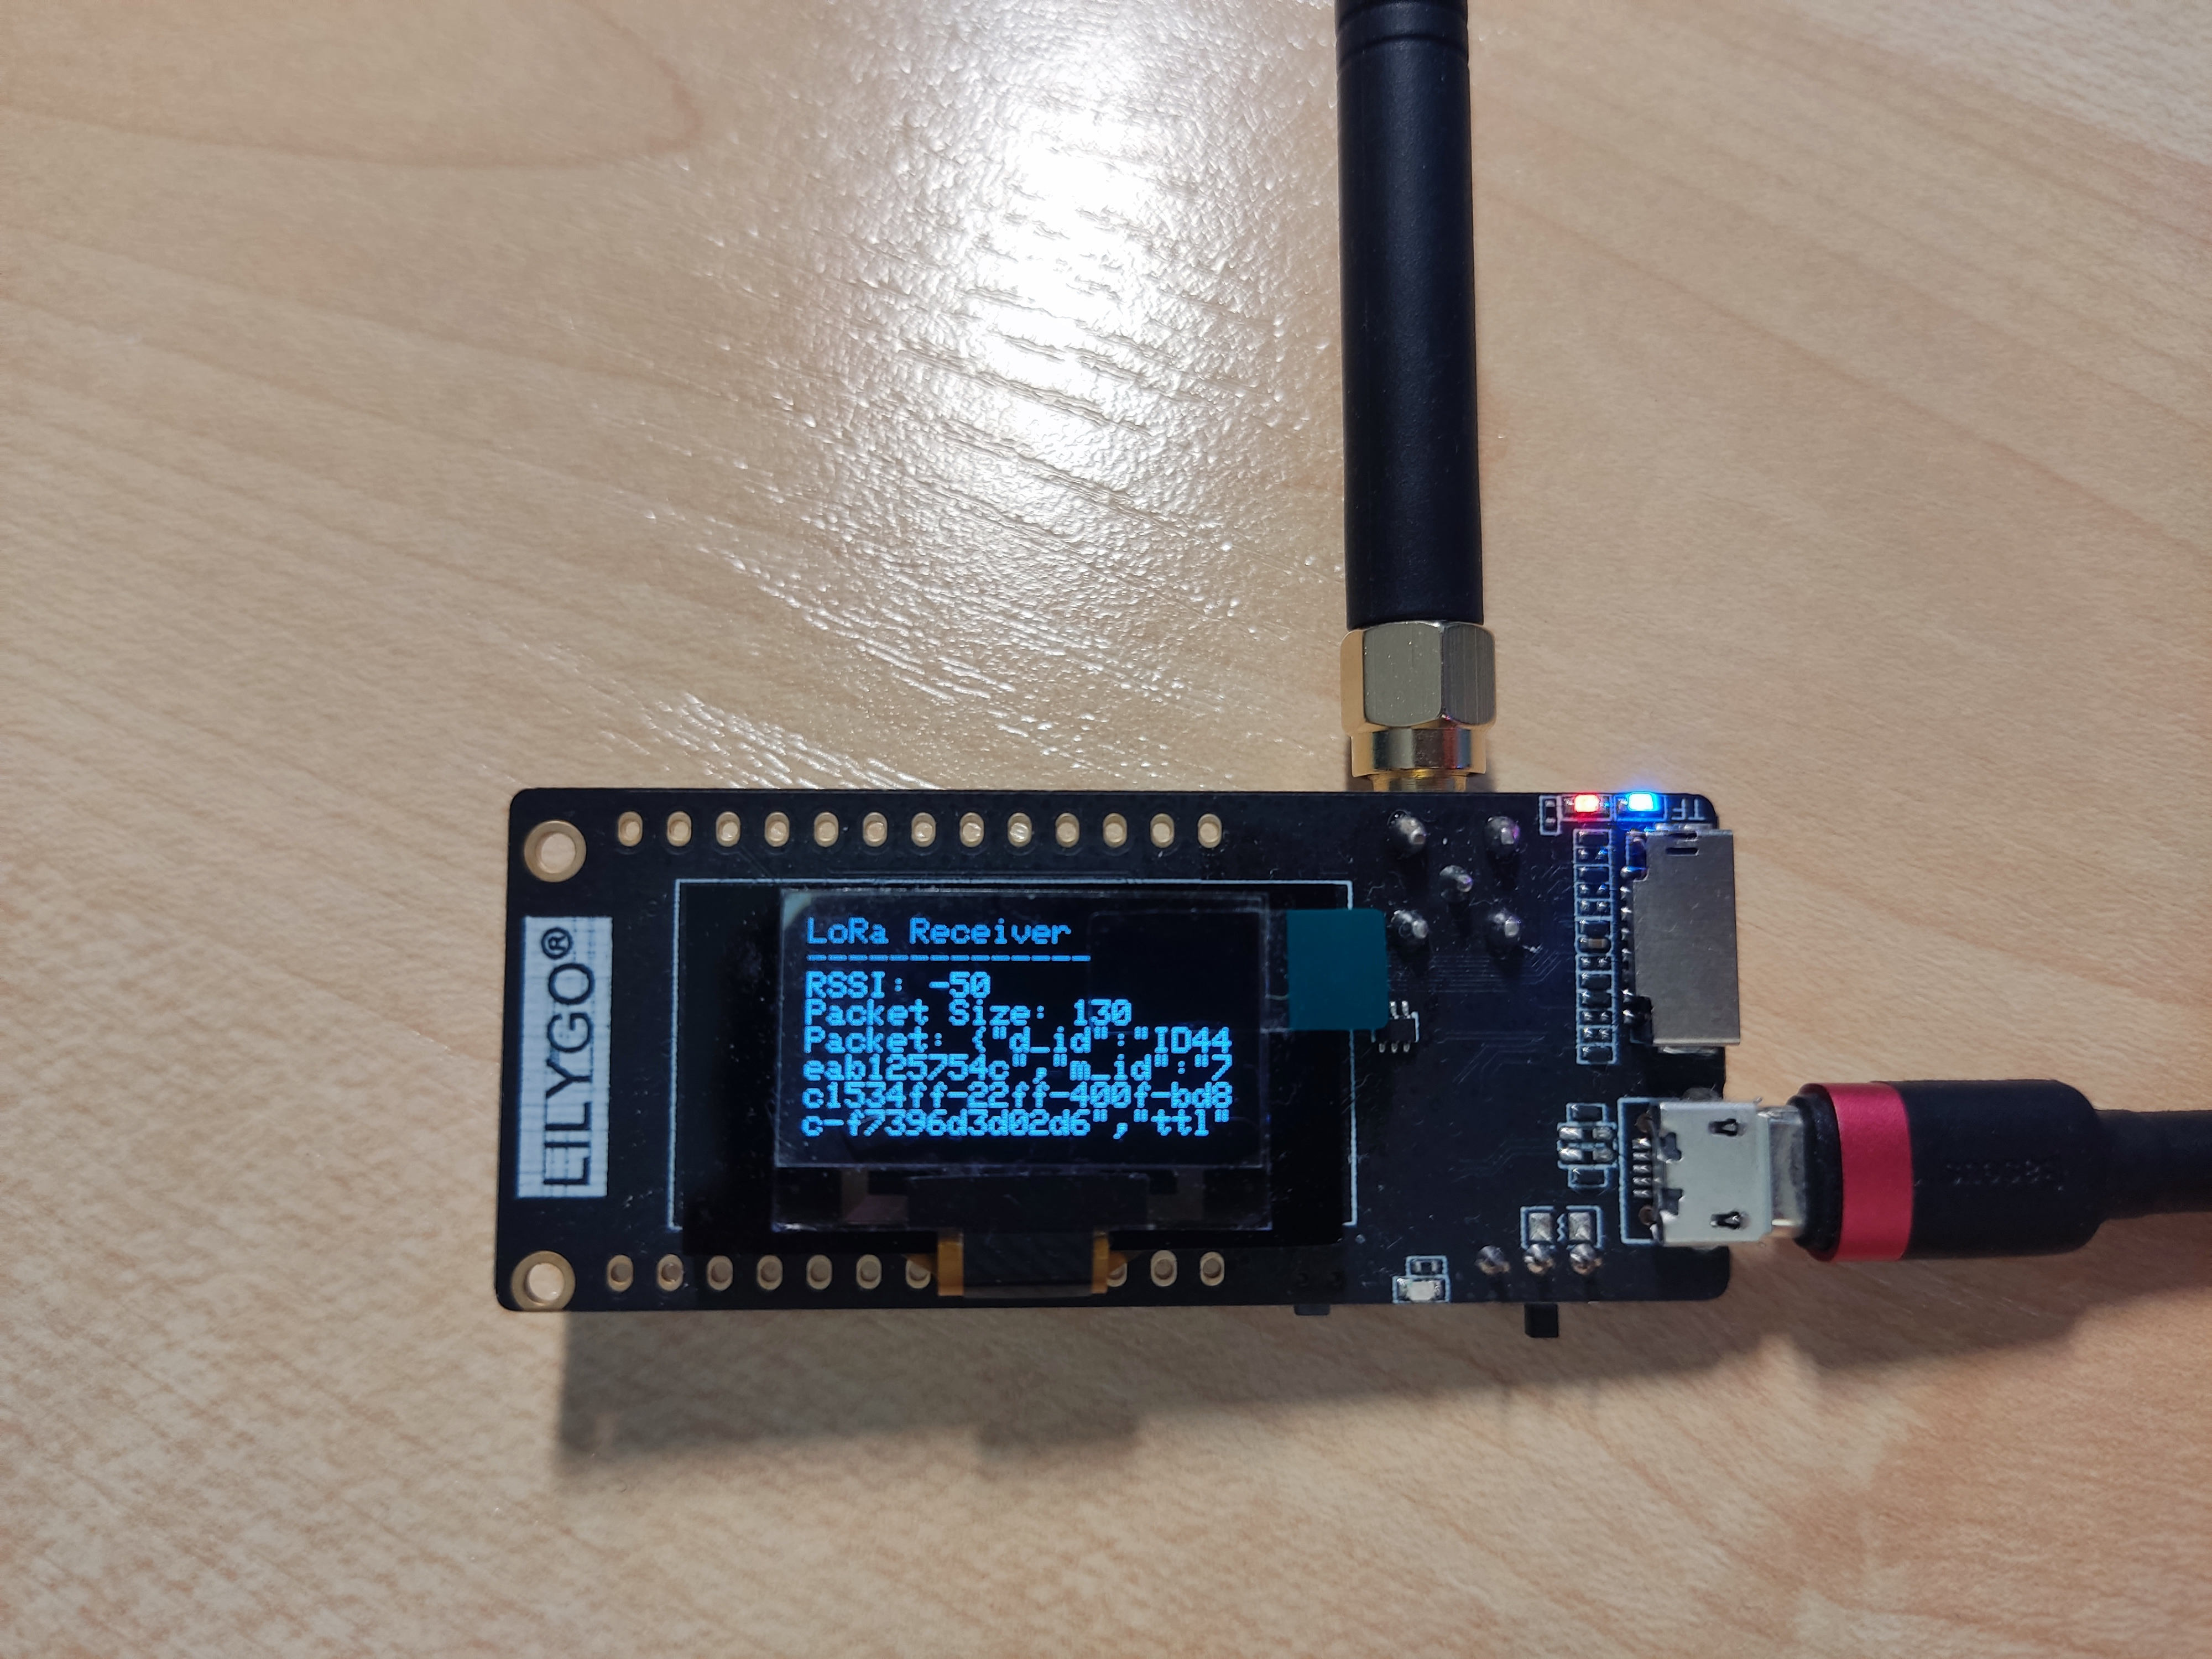
\includegraphics[width=13cm]{pic/stacja1.jpg}
    \end{center}
    \caption{Zdjęcie stacji przekaźnikowej opartej o TTGO LoRa32}\label{rys:stacja1}
\end{figure}


\subsection{Serwer testowy}
Na serwerze testowy zostały uruchomione wszystkie usługi, które zostały wykorzystane w projekcie, w szczególności:
\begin{itemize}
    \item Mosquitto
    \item InfluxDB 2
    \item Program zapisujący do InfluxDB 2
    \item Redis
\end{itemize}
Serwer został uruchomiony na maszynie wewnątrz budynku, w sieci lokalnej. Na serwerze został uruchomiony system operacyjny Debian 11. Maszyna została wyposażona w procesor Intel Core i5-480M, 2 GB pamięci RAM oraz dysk SSD o pojemności 256 GB. Wszystkie usługi zostały uruchomione w kontenerach Dockera~\cite{tools:docker}. Wszystkie usługi zostały uruchomione w jednej sieci Dockera, w celu zapewnienia komunikacji między nimi.

\subsection{Broker wiadomości}
Broker wiadomości został uruchomiony na wspólnym serwerze wewnątrz budynku. Broker został zabezpieczony hasłem, które zostało zapisane w pliku konfiguracyjnym. Wszystkie urządzenia zostały skonfigurowane tak, aby połączyć się z brokerem za pomocą tego hasła. Niestety, nie zostało użyte szyfrowanie TLS.

\subsection{Baza danych i program zapisujący dane}
Baza danych wraz z programem zapisującym dane zostały uruchomione na wspólnym serwerze wewnątrz budynku. Baza danych została zabezpieczona tokenem dostępu, który został zapisany w pliku konfiguracyjnym. Wszystkie urządzenia zostały skonfigurowane tak, aby połączyć się z bazą danych za pomocą tego tokenu. Niestety, nie zostało użyte szyfrowanie TLS. Zarówno baza danych, jak i program zapisujący dane zostały uruchomione w kontenerach Dockera, w celu zapewnienia izolacji i~łatwości konfiguracji. Na rysunku \ref{rys:influxdb-web} został przedstawiony zrzut ekranu interfejsu użytkownika InfluxDB 2. Na rysunku \ref{rys:logi-connector} został przedstawiony zrzut ekranu zawierający logi programu zapisującego pomiary do bazy InfluxDB 2.

\begin{figure}[b!]
    \begin{center}
        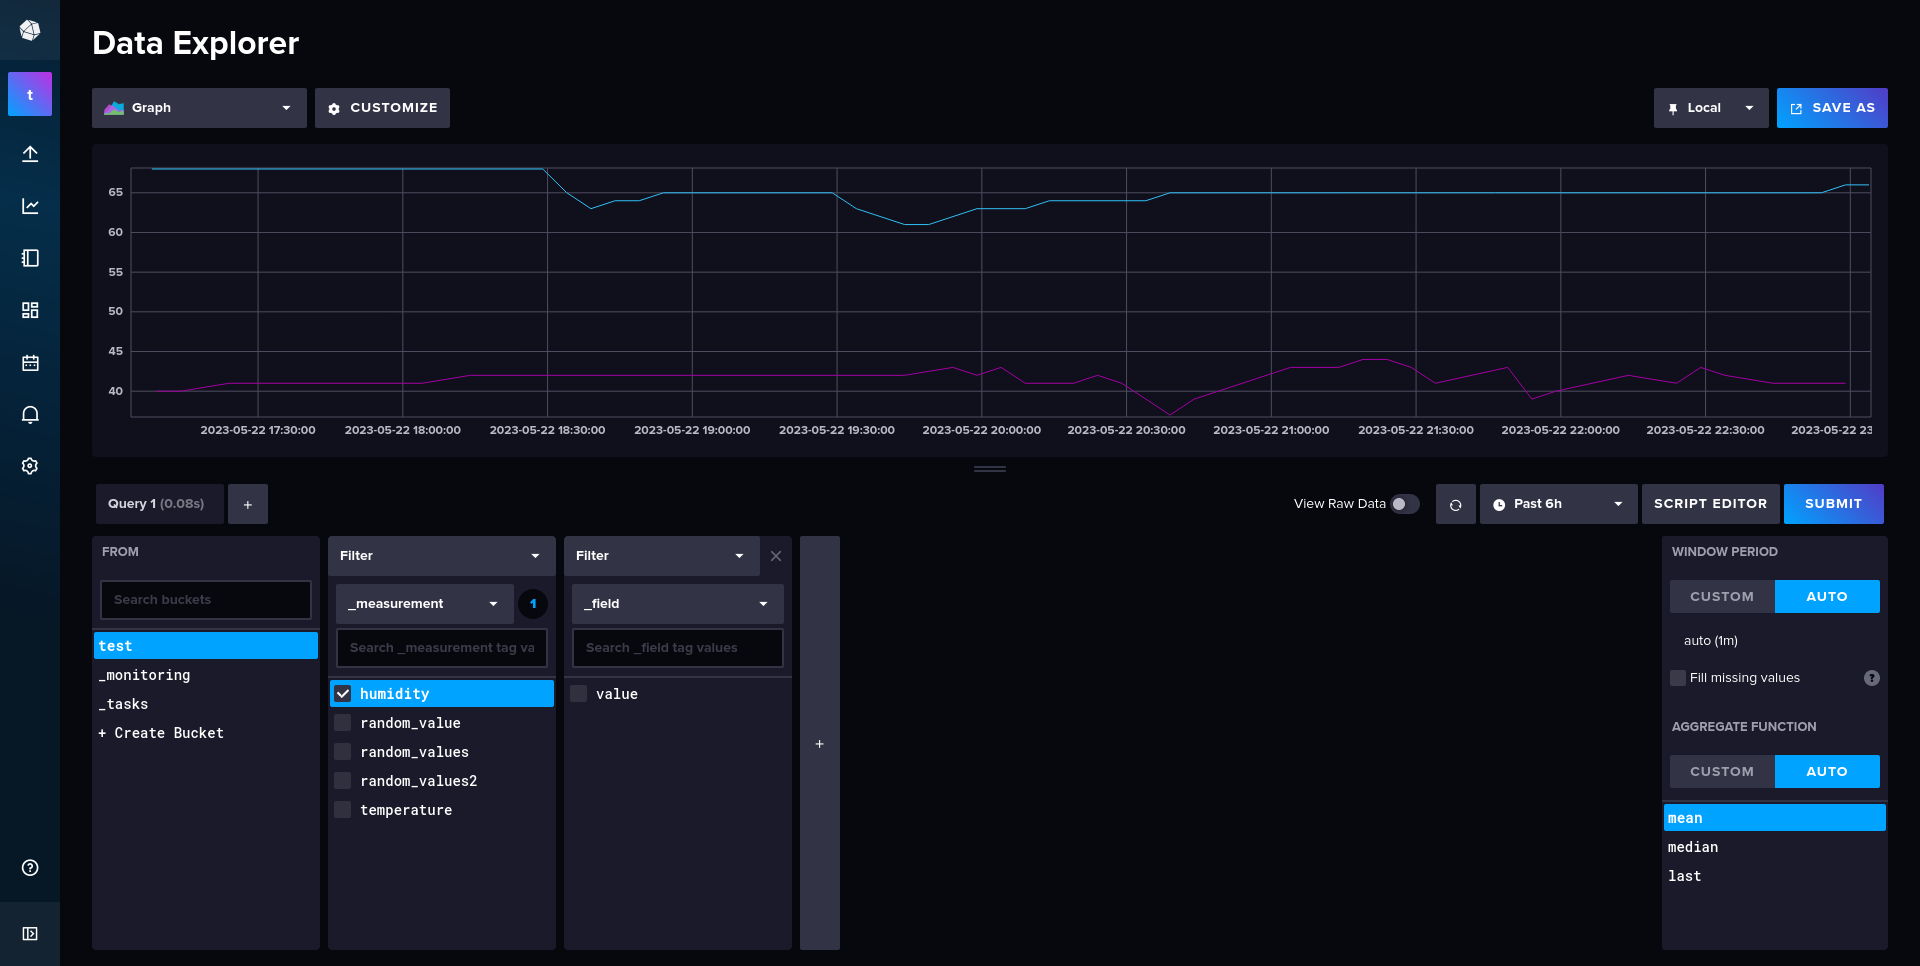
\includegraphics[width=13cm]{pic/influxdb-web.png}
    \end{center}
    \caption{Zrzut ekranu interfejsu użytkownika InfluxDB 2}\label{rys:influxdb-web}
\end{figure}

\begin{figure}[b!]
    \begin{center}
        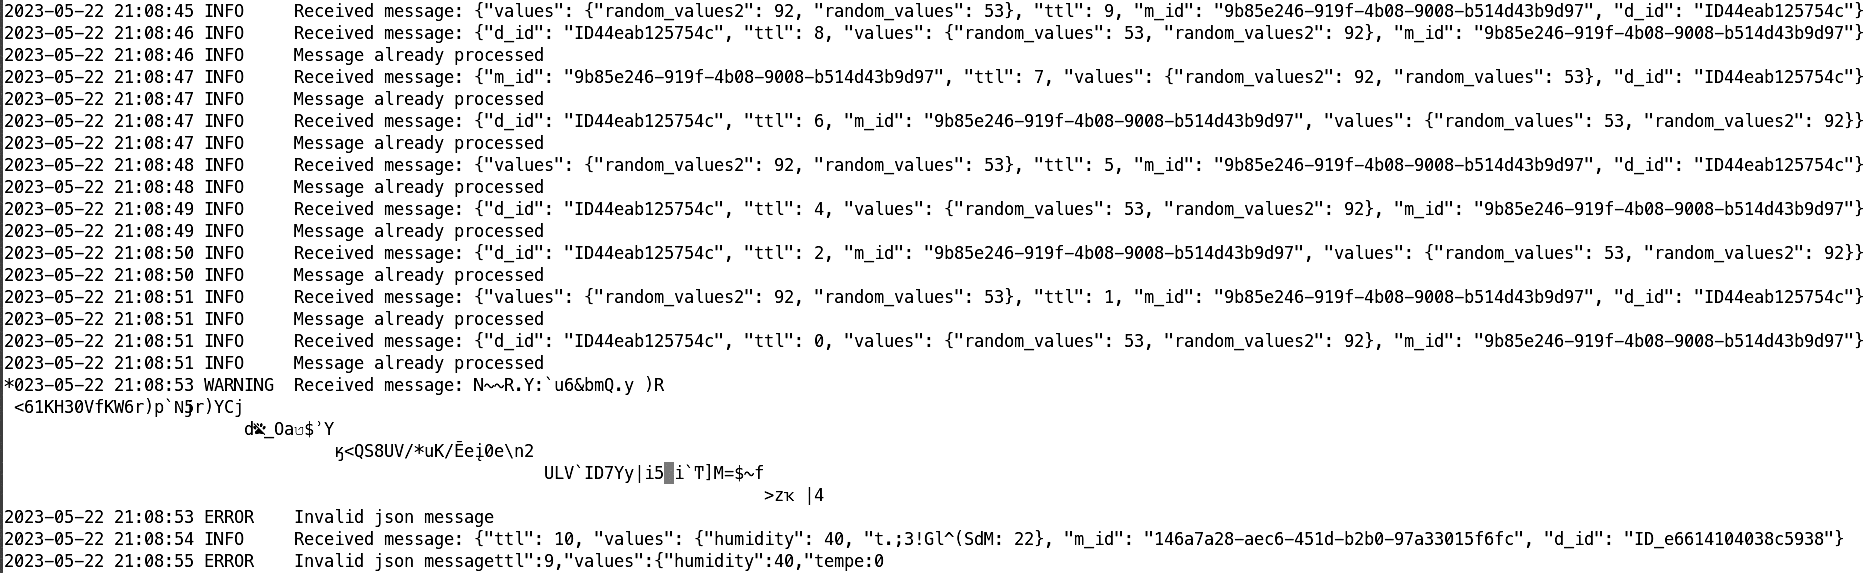
\includegraphics[width=13cm]{pic/logi-connector.png}
    \end{center}
    \caption{Zrzut ekranu zawierający logi programu zapisującego pomiary do bazy InfluxDB 2}\label{rys:logi-connector}
\end{figure}

\subsection{Redis}
Redis został uruchomiony na wspólnym serwerze wewnątrz budynku. Redis pozostał niezabezpieczony, ponieważ został udostępniony w sieci wewnętrznej. Wszystkie urządzenia zostały skonfigurowane tak, aby połączyć się z Redisem za pomocą tego hasła. Niestety, nie zostało użyte szyfrowanie TLS. Redis został uruchomiony w kontenerze Dockera, w celu zapewnienia izolacji i~łatwości konfiguracji.

% picure of server
\section{Testy}
System został przetestowany pod kątem poprawności działania, wydajności oraz niezawodności. Testy zostały przeprowadzone w dniach od 1 do 14 maja 2023 roku.

\subsection{Poprawność działania}
Poprawność działania była weryfikowań na kilka sposobów:

\subsubsection{Weryfikacja poprawności działania urządzeń pomiarowych}

Weryfikacja poprawności działania urządzeń pomiarowych została przeprowadzona dla
odczytów temperatury. Weryfikacja polegała na porównaniu odczytów z dwóch różnych czujników. Porównania dokonano pomiędzy czujnikiem \texttt{DHT11} a czujnikiem \texttt{DS18B20}. Odczyty zostały zapisane do pliku CSV a następnie porównane. Przykładowe wyniki testów zostały przedstawione na rysunku~\ref{rys:dht-vs-ds}.

\begin{figure}[b!]
    \begin{center}
        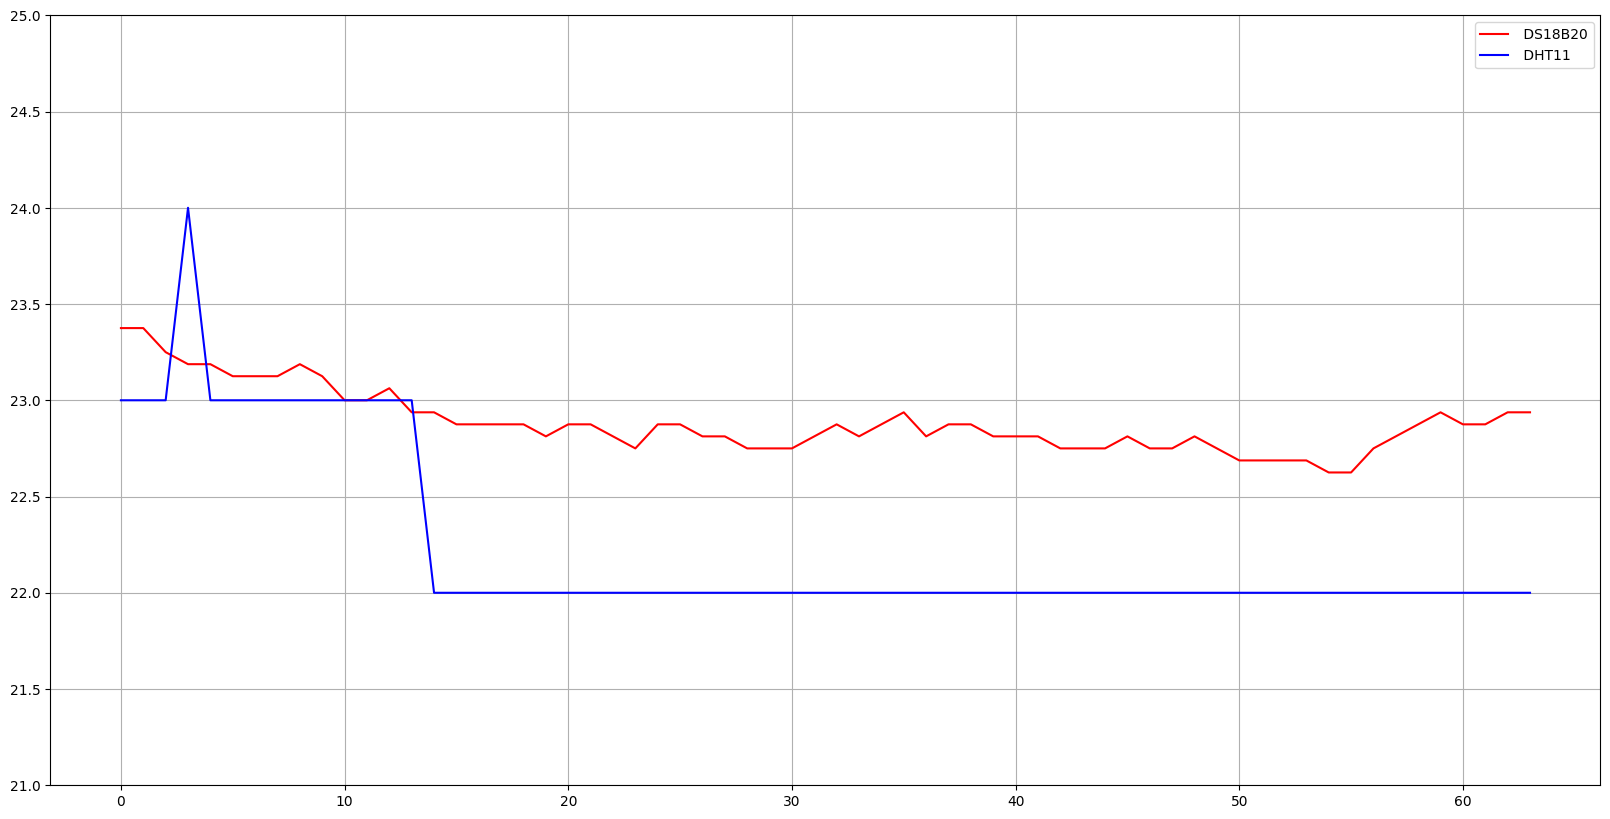
\includegraphics[width=15cm]{pic/dht-vs-ds.png}
    \end{center}
    \caption{Wykres temperatury od czasu dla czujników \texttt{DHT11} i \texttt{DS18B20}}\label{rys:dht-vs-ds}
\end{figure}

Jak widać na załączonym rysunku, wyniki odczytów są bardzo zbliżone(maksymalna różnica pomiarów to 1°C), co świadczy o poprawności działania urządzeń pomiarowych.

\subsubsection{Weryfikacja porapwności działania całego sytemu}
Weryfikacja poprawności działania całego systemu została przeprowadzona poprzez porównywanie pakietów wysyłanych przez urządzenia pomiarowe z pakietami zapisanymi w bazie danych. Weryfikacja polegała na porównaniu wszystkich pól pakietów. Porównanie to odbywało się ręcznie i dotyczyło tylko kilku pakietów. Dodatkowo weryfikowano poprawność działania poprzez sprawdzenie zmian we wskazaniach czujników. Przejścia dla temperatury i wilgotności były bardzo płynne,(co widać na rysunku) co świadczy o poprawności działania systemu. Przejścia dla liczb losowych były bardzo chaotyczne, co również świadczy o poprawności działania systemu. Przykładowe wyniki testów zostały przedstawione na rysunku~\ref{rys:porownanie-hum}.

\begin{figure}[b!]
    \begin{center}
        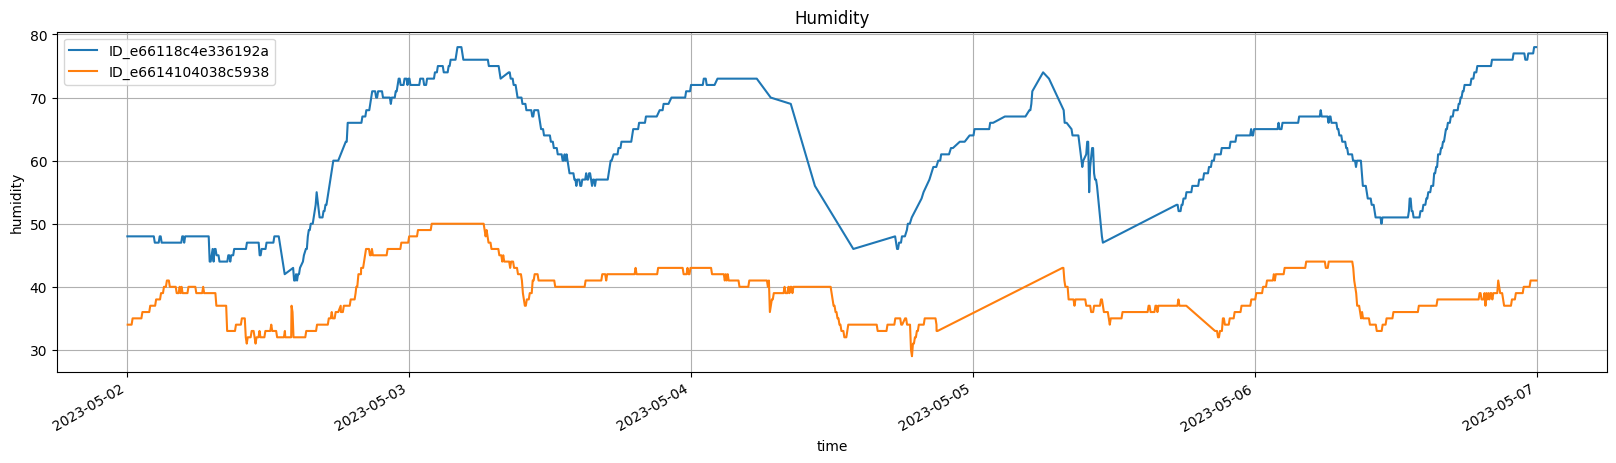
\includegraphics[width=15cm]{pic/diagram-humidity.png}
    \end{center}
    \caption{Wykres wilgotności od czasu(w okresie od 2 Maja 2023 do 7 Maja 2023)}\label{rys:porownanie-hum}
\end{figure}


Dzięki wyżej wymienionym testom, udało się stwierdzić, że system działa poprawnie.

\subsection{Wydajność}
Testy wydajności zostały przeprowadzone w celu sprawdzenia, czy system jest w stanie obsłużyć wszystkie pakiety wysyłane przez urządzenia pomiarowe. Testy zostały przeprowadzone w dwóch etapach:
\begin{itemize}
    \item Testy wydajności stacji przekaźnikowej
    \item Testy wydajności węzłów sieci
\end{itemize}

\subsubsection{Testy wydajności stacji przekaźnikowej}
Testy zostały przeprowadzone w następujący sposób: z 3 węzłów sieci były emitowane pakiety w bardzo krótkich odstępach czasu (co 10 sekund). Wszystkie pakiety były wysyłane do stacji przekaźnikowej. Następnie przekazywała ona te pakiety do brokera wiadomości. Wszystkie pakiety były zapisywane w bazie danych.

W wyniku testów zostało stwierdzone, że stacja przekaźnikowa jest w stanie obsłużyć wszystkie pakiety wysyłane przez węzły sieci poprawnie.

\subsubsection{Testy wydajności węzłów sieci}
Testy zostały przeprowadzone w następujący sposób: z 3 węzłów sieci były emitowane pakiety w bardzo krótkich odstępach czasu(10 s). Weryfikacji podlegało to, czy wszystkie pakiety zostały wysłane ponownie rozgłoszone przez węzły sieci. Wszystkie pakiety były odbierane równie przez stację przekaźnikową.

W wyniku testów zostało stwierdzone, że węzły sieci są w stanie obsłużyć wszystkie pakiety wysyłane przez sieci poprawnie. Przykładowe wyniki testów zostały przedstawione na rysunku~\ref{rys:odbijanie-pakietu}.

\begin{figure}[b!]
    \begin{center}
        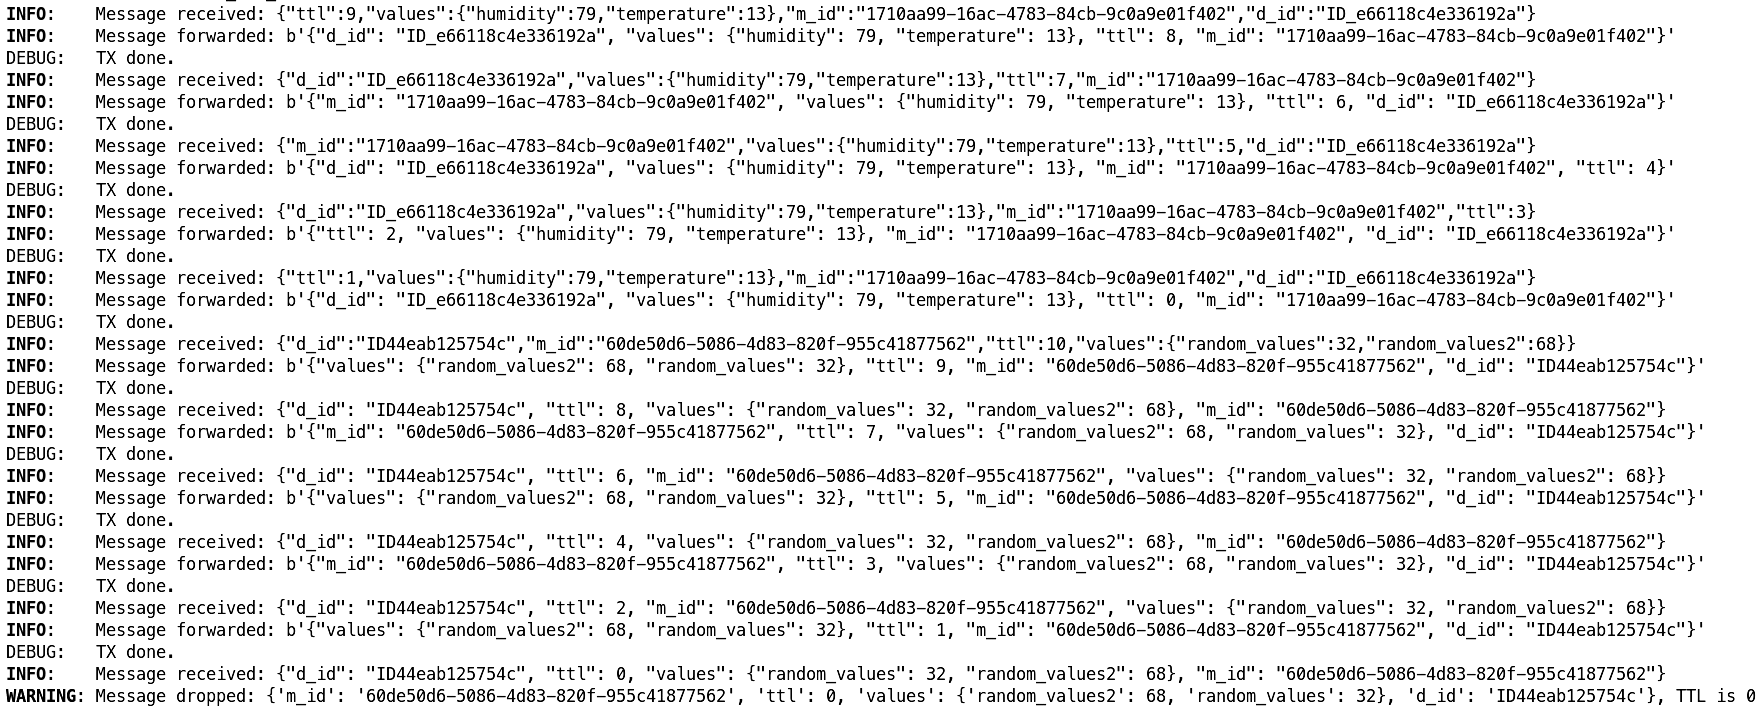
\includegraphics[width=13cm]{pic/odbijanie-pakietu.png}
    \end{center}
    \caption{Przykładowy błędny pakiet odebrany przez jeden z węzłów sieci}\label{rys:odbijanie-pakietu}
\end{figure}

\subsection{Zauważone problemy}
W trakcie testów zostały zauważone następujące problemy:
\subsubsection{Błędne pakiety}
\begin{itemize}
    \item Węzły sieci czasami odbierały błędne pakiety, jak na rysunku~\ref{rys:zly-pakiet}. Problem ten został rozwiązany prze sprawdzanie czy odebrany pakiet jest poprawny, a w przypadku błędu, pakiet jest odrzucany.
    \item Przekaźnik sieci czasami przekazuje błędne pakiety do brokera(jak na rysunku~\ref{rys:zly-pakiet}). Problem ten został rozwiązany przez sprawdzanie czy odebrany pakiet jest poprawny na poziomie programu zapisującego do bazy danych, a w przypadku błędu, pakiet jest odrzucany. Można byłoby sprawdzać poprawność pakietu na poziomie przekaźnika, ale obniżyłoby to wydajność systemu.
\end{itemize}

\begin{figure}[b!]
    \begin{center}
        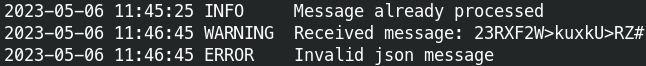
\includegraphics[width=13cm]{pic/zly-pakiet.png}
    \end{center}
    \caption{Przykładowy błędny pakiet odebrany przez jeden z węzłów sieci}\label{rys:zly-pakiet}
\end{figure}

\subsubsection{Błąd ludzki}
Jak łatwo zauważyć na wykresie~\ref{rys:diagram-scat} niestety w bazie danych pojawiają się luki w zapisanych danych. Takie luki spowodowane są brakami zasilania spowodowane przez osoby obsługujące ten system w czasie testów. Niektóre czujniki traciły zasilanie przez nieuważne zmiany kabli zasilających czy nie zmienianie baterii na czas. Jednym z możliwych rozwiązań jest zastosowanie większej baterii w każdym węźle sieci.

\begin{figure}[b!]
    \begin{center}
        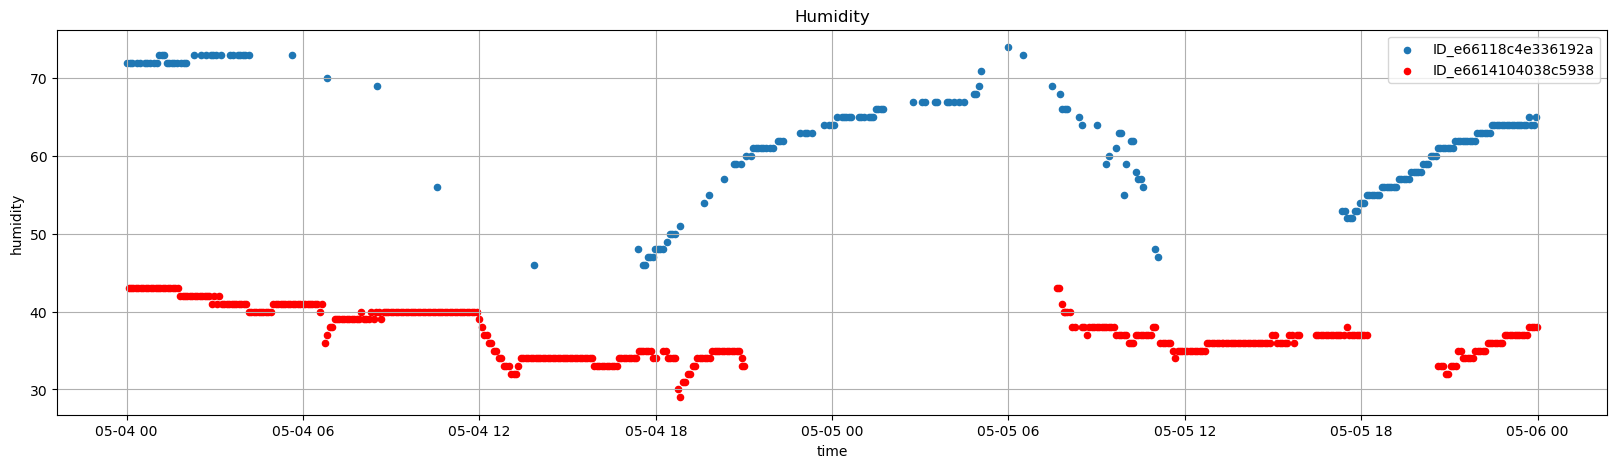
\includegraphics[width=13cm]{pic/diagram-scat-humm.png}
    \end{center}
    \caption{Szczegółowych diagram danych zapisanych w bazie między 4 Maja, a 6 Maja 2023}\label{rys:diagram-scat}
\end{figure}

%  TODO: add more screenshots
